% !TeX program = lualatex
% ---------------------------------------------------------------
%  Stuurmanskonst — Samarang, 1787
%  Nationaal Archief 1.04.02, inv. 3775, fol. 3614–3616
%  GLOBALISE scans 0048–0050
%
%  Companion to geometria.tex, from the same submission: the ten
%  examples of the navigation section, seven folios after the
%  geometry ends.
%
%      lualatex stuurmanskonst.tex
%
%  Self-contained: enumitem.sty and needspace.sty are vendored beside
%  this file (TeX Live "basic" ships neither), and EB Garamond lives in
%  fonts/ as the OFL variable faces, so no system install is needed.
% ---------------------------------------------------------------
\documentclass[11pt,twoside,openany]{book}

\usepackage{fontspec}
\usepackage{amsmath,amssymb}
\usepackage{tikz}
\usepackage[a4paper,inner=28mm,outer=24mm,top=26mm,bottom=26mm]{geometry}
\usepackage{xcolor}
\usepackage{enumitem}
\usepackage{fancyhdr}
\usepackage{needspace}
% Lets \footnote survive being written inside a box: see \wnote below.
\usepackage{footnote}
\usepackage{microtype}
\usepackage[hidelinks]{hyperref}

\setmainfont{EBGaramond-var.ttf}[
  Path              = ./fonts/,
  UprightFeatures   = {RawFeature={axis={wght=400}}},
  ItalicFont        = EBGaramond-Italic-var.ttf,
  ItalicFeatures    = {RawFeature={axis={wght=400}}},
  BoldFont          = EBGaramond-var.ttf,
  BoldFeatures      = {RawFeature={axis={wght=700}}},
  BoldItalicFont    = EBGaramond-Italic-var.ttf,
  BoldItalicFeatures= {RawFeature={axis={wght=700}}}]

% Vulgar fractions. EB Garamond builds these from a plain solidus via the
% OpenType `frac` feature; a literal U+2044 does not trigger it, so halves
% must be written \vfrac{1}{2} and never with a fraction slash.
\newcommand{\vfrac}[2]{{\addfontfeature{Fractions=On}#1/#2}}

% Degrees and minutes. The second argument is set in text so that it can
% carry a \vfrac: the manuscript writes 36½ and 00½ with a vulgar half.
\newcommand{\ang}[2]{$#1^{\circ}$\,#2$'$}

\definecolor{msred}{HTML}{8A3324}
\definecolor{msink}{HTML}{211E1A}
\definecolor{msmut}{HTML}{6B6357}
\definecolor{msfaint}{HTML}{9A9388}
\definecolor{msrule}{HTML}{DCD3C2}
\definecolor{mscream}{HTML}{F5F0E4}
\color{msink}

\setlength{\parindent}{0pt}
\setlength{\parskip}{0pt}
\pagestyle{fancy}\fancyhf{}
\renewcommand{\headrulewidth}{0pt}
\fancyfoot[LE,RO]{\color{msfaint}\footnotesize\thepage}
\fancyfoot[C]{\color{msfaint}\scriptsize\MakeUppercase{Stuurmanskonst \textperiodcentered\ Samarang, 1787}}

\newcommand{\rubric}[1]{{\color{msred}\scriptsize\MakeUppercase{#1}}\par\vspace{3pt}}

\newcommand{\exempel}[2]{%
  \par\vspace{16pt}\needspace{4\baselineskip}%
  \noindent\begin{minipage}{\linewidth}
    {\large #1}\hfill{\color{msfaint}\scriptsize\MakeUppercase{#2}}\par
    \vspace{3pt}{\color{msrule}\hrule height 0.4pt}
  \end{minipage}\par\vspace{10pt}}

\newcommand{\foliomark}[3]{%
  \par\vspace{10pt}\noindent{\color{msfaint}\scriptsize
  \MakeUppercase{Folio #1 \textperiodcentered\ scan #2}\hfill\MakeUppercase{Examples #3}}\par
  \vspace{2pt}{\color{msrule}\hrule height 0.4pt}\par\vspace{4pt}}

\newcommand{\foliostand}[2]{\par\vspace{6pt}{\color{msred}\large #1}\par
  \vspace{4pt}{\color{msmut}\footnotesize #2}\par\vspace{6pt}}

\newcommand{\dutchtext}[1]{\rubric{Dutch --- as written}{\fontsize{12.5}{16}\selectfont #1}\par\vspace{10pt}}

\newcommand{\engtext}[1]{%
  \noindent\begin{minipage}{\linewidth}
    {\color{msrule}\vrule width 1.5pt}\hspace{8pt}%
    \begin{minipage}{\dimexpr\linewidth-16pt\relax}
      \rubric{English}{\color{msmut}\small #1}
    \end{minipage}
  \end{minipage}\par\vspace{12pt}}

\newcommand{\worktitle}[2]{\par\vspace{12pt}\needspace{5\baselineskip}%
  {\color{msred} #1}\hfill{\color{msfaint}\scriptsize\MakeUppercase{#2}}\par
  \vspace{2pt}{\color{msrule}\hrule height 0.4pt}\par\vspace{8pt}}

\newenvironment{workblock}{\begin{list}{}{\setlength{\leftmargin}{0pt}\setlength{\itemsep}{3pt}\setlength{\parsep}{0pt}}}{\end{list}}

% The label column wraps rather than overflows: \makebox neither wraps nor
% shrinks, so a label wider than 22mm would grow leftward into the margin.
%
% savenotes wraps the whole row, not the note column: a \footnote written
% inside a minipage sets there as a lettered note with its own rule, which
% forces the box open and drives the working's lines apart. Held and emitted
% outside the boxes, the note goes to the foot of the page where its mark is
% and the rows keep their spacing. Six of these rows carry a footnote.
\newcommand{\wrow}[3]{\item[]\begin{savenotes}%
  \parbox[t]{22mm}{\raggedleft\color{msmut}\itshape\small #1\strut}\hspace{5mm}%
  \begin{minipage}[t]{58mm}#2\end{minipage}%
  \hspace{5mm}\begin{minipage}[t]{\dimexpr\linewidth-90mm\relax}{\color{msmut}\footnotesize #3}\end{minipage}%
  \end{savenotes}}

% A row whose first element is not a gutter label but a rule stated in words,
% too long for \wrow's 22mm label column: it is set on its own line, indented
% to the working column, with the figures beneath it.
\makeatletter
\newcommand{\wprop}[2]{%
  \item[]\hspace*{27mm}%
  \begin{minipage}[t]{\dimexpr\linewidth-27mm\relax}\raggedright
    {\color{msmut}\itshape\small #1}\par\vspace{3pt}#2\par\vspace{2pt}%
  \end{minipage}}
\makeatother

\newcommand{\ruleunder}{\par\vspace{2pt}\hspace*{27mm}{\color{msink}\hrule height 0.9pt width 58mm}\vspace{2pt}}

% \parbox, not minipage: minipage diverts \footnote into the box, where it
% sets as a lettered note with its own rule. savenotes then holds each note
% and emits it outside the box, on the page where its mark stands.
\newcommand{\wnotebox}[1]{\parbox[t]{\dimexpr\linewidth-27mm\relax}{%
  \raggedright\setlength{\parskip}{4pt}\setlength{\parindent}{0pt}#1}}
\newcommand{\wnote}[1]{\item[]\hspace*{27mm}%
  \begin{savenotes}\wnotebox{#1}\end{savenotes}}

% The heading that falls inside the section, before the sixth example.
\newcommand{\mssection}[2]{\par\vspace{16pt}\needspace{5\baselineskip}%
  {\color{msred}\large #1}\par\vspace{3pt}
  {\color{msmut}\footnotesize #2}\par\vspace{5pt}
  {\color{msred}\hrule height 0.5pt width 4cm}\par\vspace{2pt}}

\newcommand{\reading}[1]{\par\vspace{12pt}\rubric{Reading}{\small #1}\par\vspace{8pt}}

% The cream panel is captured in a box: \colorbox needs its argument as one
% group, which cannot straddle an environment's begin and end parts.
\newsavebox{\msfigbox}
\newenvironment{msfigure}{\par\vspace{6pt}\begin{center}\setlength{\fboxsep}{10pt}%
  \begin{lrbox}{\msfigbox}\begin{minipage}{\dimexpr0.62\linewidth-20pt\relax}\centering}%
  {\end{minipage}\end{lrbox}\colorbox{mscream}{\usebox{\msfigbox}}\end{center}\par\vspace{8pt}}
\newcommand{\mscaption}[1]{\par\vspace{6pt}{\color{msmut}\scriptsize #1}}

\newlist{msnotes}{description}{1}
\setlist[msnotes]{font=\color{msred}\normalfont\scriptsize,leftmargin=12pt,itemsep=2pt,topsep=6pt,before=\scriptsize\color{msmut}}

% Both kinds of figure in the section are the same circle — a great circle of
% the sphere seen edge-on, lettered round its rim: the meridian for the first
% seven questions, the horizon for the last three. Angles are reckoned from
% the right-hand point counter-clockwise, so on the meridian a star's angle is
% its altitude above N, and on the horizon a bearing's angle is its amplitude
% north of east.
%
% The equator is square to the polar axis, NOT its mirror in the vertical: at
% latitude phi the pole stands phi above the horizon and the equator 90-phi
% above the opposite point. Pass both angles; do not derive one from the other.
\newcommand{\mscircle}{\draw[msink,thick] (0,0) circle (2.6);
  \draw[msink] (-2.6,0) -- (2.6,0);\draw[msink] (0,-2.6) -- (0,2.6);}
\newcommand{\msdiam}[1]{\draw[msink] (#1:2.6) -- (#1+180:2.6);}
\newcommand{\mschord}[2]{\draw[msink,dashed] (#1:2.6) -- (#2:2.6);}
\newcommand{\msarc}[2]{\draw[msred,line width=1.6pt] (#1:2.6) arc (#1:#2:2.6);}
\newcommand{\msdot}[1]{\fill[msink] (#1:2.6) circle (0.075);}
% Optional radius pushes a label clear of its neighbour where two points fall
% within a few degrees of each other, as they do at high and low latitudes.
\newcommand{\mslab}[3][2.95]{\node at (#2:#1) {\small #3};}

\begin{document}
\frontmatter
\thispagestyle{empty}
\vspace*{0.12\textheight}
{\color{msred}\scriptsize\MakeUppercase{Nationaal Archief 1.04.02 \textperiodcentered\ inv. 3775}}\par
\vspace{4pt}{\color{msred}\hrule height 0.8pt}\par
\vspace{0.20\textheight}
{\color{msmut}\small\MakeUppercase{Zeevaartkundige Examens}}\par\vspace{20pt}
{\color{msred}\fontsize{52}{52}\selectfont Stuurmanskonst}\par\vspace{20pt}
{\large Ten examination questions on the latitude, the hour and the error of the compass, with the examiner's own model answers, from the marine school at Samarang.}\par
\vspace{22pt}{\color{msrule}\hrule height 0.4pt width 5.5cm}\par\vspace{16pt}
{\color{msmut}\small Diplomatic text from the manuscript, with translation,\\reconstructed figures and commentary.\\Folios 3614--3616 \textperiodcentered\ GLOBALISE scans 0048--0050.}\par
\vfill
{\color{msfaint}\footnotesize A companion piece to \textit{Geometria}, from the same submission. The machine transcription of the VOC archive has been corrected throughout against the scans, and every figure recomputed.}\par
\clearpage

\chapter*{A later section of the same paper}
The examination paper edited in \textit{Geometria} does not end with its thirtieth geometrical example. It is a submission in sections, one to each subject: the geometry is the first, and the volume runs on through rectilinear trigonometry, gunnery and the mensuration of shot-piles to the section edited here --- \textit{Stuurmanskonst}, the steersman's art --- at fol.~3614, seven folios beyond the end of the geometry.\footnote{Scan and folio do not run together, a blank leaf between the sections being left unnumbered: scan 0040 is fol.~3607, where the geometry ends, and scan 0048 is fol.~3614.}\par\vspace{8pt}
The heading stands in two lines: \textit{Stuurmanskonst} across the top of the leaf and, beneath it, the section proper --- \textit{Van de Sons en Sterre Hoogmeeting}, of the measuring of the height of the sun and stars. Ten examples follow, over three folios, and a second heading at the ninth of them, \textit{Van het Verbeeteren der Zons Declinatie}, marks where the subject turns. The section closes with the tenth; a third heading, \textit{van de Zeijlagie}, opens the sailings on the next leaf and takes the numbering on to the eleventh.\par\vspace{8pt}
The form is unchanged from the geometry: the examiner sets the question and answers it himself, the figure is drawn small in the margin at the left and the working set out to the right in a column. What has changed is the figure. It is one circle, lettered round its rim --- the plane of the observer's meridian for the first seven questions, the plane of his horizon for the last three --- and almost every question in the section is answered by reading arcs off it.

\chapter*{How this edition was made}
{\color{msred}\large 1 \textperiodcentered\ Correction against the scans}\par\vspace{4pt}
Every line printed here has been re-read from the images. The machine transcription fails on the lettered arcs, which are the whole content of the working --- BP comes out as \texttt{88}, TM$+$BN as \texttt{TTABNI}, PN as \texttt{xW} --- and it returns each page's lines in the order the layout analysis found them rather than in reading order, so on the first leaf both headings and the first example's answer arrive at the very end, after the second example. Where the machine reading is instructive it is quoted in the notes, in a monospaced face.\par\vspace{10pt}
{\color{msred}\large 2 \textperiodcentered\ Verification of the arithmetic}\par\vspace{4pt}
Every working has been recomputed line by line. All ten are internally exact: no subtraction, division, proportion or logarithm on these three folios is wrong. Two examples round, and the notes say by how much.\par\vspace{10pt}
{\color{msred}\large 3 \textperiodcentered\ Verification of the tables}\par\vspace{4pt}
The workings open from tables --- polar distances, right ascensions, the sun's declination --- and those are checkable against the sky. The stars have been reduced to the mean equator and equinox of the year each question names, from modern positions with proper motion applied, and the sun computed for the day. The examiner's figures stand up: his sun is right to a minute or two throughout, and his log tangents to all five places he gives. This test settles the one disputed reading on the first leaf, and it is what uncovers the fault described in \S5.\par\vspace{10pt}
{\color{msred}\large 4 \textperiodcentered\ Figures}\par\vspace{4pt}
The seven circles are redrawn after the marginal originals, keeping the manuscript's lettering and its construction, and set to the figures each example answers --- which is what the scribe himself does, and the reason no two of his circles look alike. They are not facsimiles. The arcs the working turns on are marked in red; the manuscript marks them, less legibly, with broken chords.\par\vspace{10pt}
{\color{msred}\large 5 \textperiodcentered\ An error in the specimen}\par\vspace{4pt}
Recomputation turned up one substantive fault, and since the document is an answer key it is the examiner's own. \textcolor{msred}{The workings of the third and fourth examples are transposed.} Both ask for the hour at which a named star crosses the meridian of Samarang, on two different dates. The third example asks for Arcturus on 1 September and is answered from the right ascension of Antares and the sun's place on 16 August; the fourth asks for Antares on 16 August and is answered from the right ascension of Arcturus and the sun's place on 1 September. Neither working contains an arithmetical error, and each is right --- for the other question. The answers went to Amsterdam attached to the wrong questions. The figures are set out in the note to the third example.

\clearpage
\pagenumbering{arabic}

\foliomark{3614}{0048}{1--2}
\foliostand{The steersman's art \textperiodcentered{} finding the latitude from the height of a star}{The section opens on a recto, the verso facing it left blank. The old pagination \textit{25} stands beneath the archival foliation at the head and is struck through.}

% ---------------------------------------------------------------
\exempel{1ste Exempel}{First Example}

\begin{msfigure}
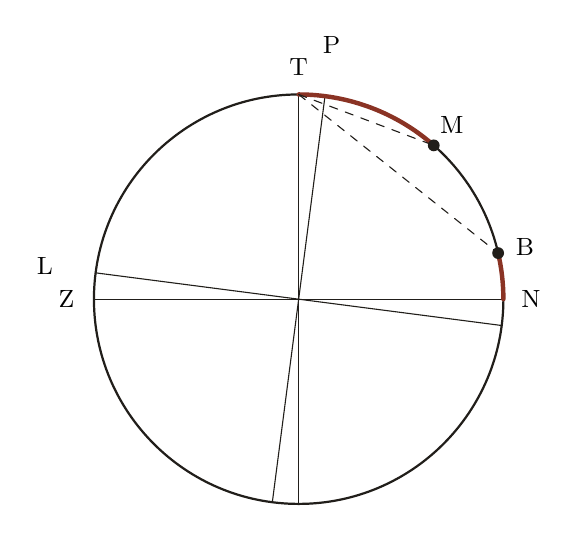
\begin{tikzpicture}[line cap=round,line join=round]
  \mscircle \msdiam{82.61} \msdiam{172.61}
  \msarc{48.71}{90} \msarc{0}{13.01}
  \mschord{90}{48.71} \mschord{90}{13.01}
  \msdot{48.71} \msdot{13.01}
  \mslab{0}{N} \mslab{180}{Z} \mslab{90}{T}
  \mslab[3.25]{82.61}{P} \mslab[3.25]{172.61}{L}
  \mslab{48.71}{M} \mslab{13.01}{B}
\end{tikzpicture}
\mscaption{Redrawn after the marginal figure, at the latitude it answers. Z and N are the south and north points of the horizon, T the \textit{toppunt} or zenith; P is the pole, standing above N by the latitude, and L the equator --- \textit{de Linie} --- crossing above Z by its complement. B is Arcturus and M the middle horse, each at its lowest in the north; the red arcs TM and BN are the working's two unknowns.}
\end{msfigure}

\dutchtext{Anno 1782, word Bootes de Boer,\footnote{\textit{Bootes de Boer} --- Bo\"otes the Ploughman, the manuscript glossing the constellation in Dutch and then naming its chief star. \textit{Het middelste paard van de groote Wagen} is the middle of the three stars that draw the Great Wagon: our Mizar.} off Arcturius, Als hij op 't Laagste is, 28 grade 17 minute, verder Benoorden het toppunt geschooten, als het middelste paard van de groote Wagen, als hij op het Laast\footnote{\textit{Op het Laast} --- at his last, that is at lower culmination; \textit{op 't Laagste} in the same sentence says the same of Arcturus. \textit{Geschooten}, ``shot'', is the ordinary word for taking an altitude.} in 't Noorden bovende Horizond staad; vrage op wat Breete dit zoude Weesen. \textcolor{msred}{Antwoord, op 82 gr:\ 36\vfrac{1}{2} men:\ Noorder Breete.}}
\engtext{In the year 1782 Bo\"otes the Ploughman, or Arcturus, at his lowest, is shot 28 degrees 17 minutes further north of the zenith than the middle horse of the Great Wagon stands above the horizon at his lowest in the north; asked, what would the latitude be? \textit{Answer: 82 degrees 36\vfrac{1}{2} minutes north latitude.}}

\worktitle{Bewerking}{Working}
\begin{workblock}
  \wrow{}{\ang{69}{36} $=$ BP}{Arcturus's distance from the pole.}
  \wrow{}{\ang{33}{54} $=$ MP}{The middle horse's distance from the pole.}\ruleunder
  \wrow{}{\ang{35}{42} $=$ MB}{The arc between the two stars.}
  \wrow{}{\ang{90}{00} $=$ TN}{Zenith to the north point of the horizon.}\ruleunder
  \wrow{}{\ang{54}{18} $=$ TM $+$ BN}{What the quadrant has left once MB is taken out of it.\footnote{T, M, B and N lie in that order on the meridian, so TM $+$ MB $+$ BN makes up the quadrant TN. The examiner does not say so. His sign for \textit{plus} here is a heavy quatrefoil cross, set as $+$ throughout.}}
  \wrow{Substr.}{\ang{28}{17} $=$ TM $-$ BN}{The observation.\footnote{The question states Arcturus's distance north of the zenith less the middle horse's height above the horizon, TB $-$ MN. MB lies inside both differences and cancels from each, so TM $-$ BN is the same number; the examiner substitutes it without comment.}}\ruleunder
  \wrow{}{\ang{26}{01} $=$ 2 BN}{Sum less difference leaves twice the lesser arc.}\ruleunder
  \wrow{2 $\big)$}{\ang{13}{00\vfrac{1}{2}} $=$ BN}{The height of Arcturus at his lowest.}
  \wrow{}{\ang{69}{36} $=$ PB}{His distance from the pole again, the letters unordered.}\ruleunder
  \wrow{NP $=$}{\ang{82}{36\vfrac{1}{2}} $=$ Noorder Breete}{The pole above the horizon, which is the latitude.}
\end{workblock}

\reading{The whole of it is arcs of one circle, taken in and out of a quadrant. Two are known from a table --- the polar distances of Arcturus and of Mizar --- and their difference is the arc MB standing between the two stars. Take that out of the quadrant TN and what is left is TM and BN added together; the observation gives the same two subtracted; and sum and difference then yield each. The lesser, BN, is Arcturus's height above the north point at his lowest, and adding his distance from the pole raises the pole itself above the horizon, which is the latitude. Nothing is measured but the one angle of \ang{28}{17}.}

\begin{msnotes}
  \item[2.] Reduced to the equinox of 1782, Arcturus's polar distance was \ang{69}{40.5} and Mizar's \ang{33}{55.9}: the table is low by four and a half minutes on the first and by two on the second. Carried through the same working they give \ang{82}{39.7}, three minutes from his answer and all of it inherited from the table.
  \item[10.] \ang{82}{36\vfrac{1}{2}} north is beyond any latitude reached by 1782 --- Phipps had been stopped by the ice at \ang{80}{48} in 1773. The examiner chose his \ang{28}{17} to make the halving come out even, and the wording concedes it: \textit{dit zoude Weesen}, what this \textit{would} be. The machine transcription reads the line \texttt{op 32 gr:„ 3672 men„ Noorder Boete}, and returns it, with the two headings, at the very end of the page.
\end{msnotes}

% ---------------------------------------------------------------
\exempel{2de Exempel}{Second Example}

\begin{msfigure}
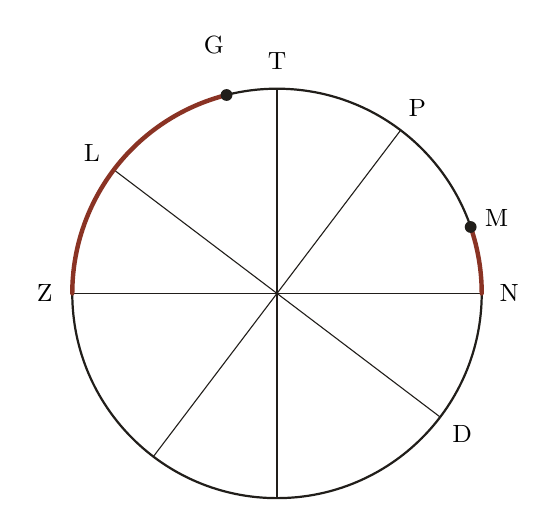
\begin{tikzpicture}[line cap=round,line join=round]
  \mscircle \msdiam{52.85} \msdiam{142.85}
  \msarc{104.27}{180} \msarc{0}{18.93}
  \msdot{104.27} \msdot{18.93}
  \mslab{0}{N} \mslab{180}{Z} \mslab{90}{T}
  \mslab{52.85}{P} \mslab{142.85}{L} \mslab{322.85}{D}
  \mslab[3.25]{104.27}{G} \mslab{18.93}{M}
\end{tikzpicture}
\mscaption{The same circle at the latitude of the second example. G is the Vulture --- Vega --- at her highest in the south, M the middle horse at his lowest in the north; the red arcs are their heights ZG and MN, the one four times the other.}
\end{msfigure}

\dutchtext{Anno 1780, zeekere stuurman, schiet de gier off\ Lijra,\footnote{\textit{De gier} --- the Vulture, the Dutch star-name that the manuscript at once glosses with the constellation, \textit{Lijra}; the star is Vega. \textit{Zeekere stuurman}, ``a certain steersman'', marks the observation as one actually made.} in het zuijden op zijn hoogste, en vind de zelve viermaal zoo hoogte staan, als het middelste paard van de groote waagen, in het Noorden op zijn Laagste staad; vrage op wat Breete zulks geschiet is ---}
\engtext{In the year 1780 a certain steersman shoots the Vulture, or Lyra, in the south at her highest, and finds her standing four times as high as the middle horse of the Great Wagon at his lowest in the north; asked, in what latitude did this happen? ---}

\worktitle{Bewerking}{Working}
\begin{workblock}
  \wrow{}{\ang{51}{36} $=$ PG}{The Vulture's distance from the pole.\footnote{The digit is a 3, formed as in the 33 written beneath it --- but the sum on the next line is taken from \ang{51}{26}, which is what Vega's polar distance actually was. See the note below.}}
  \wrow{}{\ang{33}{55} $=$ PM}{The middle horse's distance from the pole.}\ruleunder
  \wrow{}{\ang{85}{21} $=$ GM}{Star to star, across the pole.}
  \wrow{}{\ang{180}{00} $=$ ZTN}{The whole meridian, south point to north point.}\ruleunder
  \wrow{5 $\big)$}{\ang{94}{39} $=$ ZG $+$ MN}{What is left of it: the two heights together.}\ruleunder
  \wrow{}{\ang{18}{56} $=$ MN}{One part in five --- \ang{18}{55.8}, taken to \ang{18}{56} --- the observation making the other four.}
  \wrow{}{\ang{33}{55} $=$ PM}{The middle horse's distance from the pole again.}\ruleunder
  \wrow{}{\ang{52}{51} $=$ PN}{\textit{off de Noorder polus hoogte} --- or the height of the north pole.}
\end{workblock}

\reading{Where the first example worked in a quadrant, this one works in the whole semicircle. G, P, M and N follow one another round the meridian from the zenith northward, so GM is the two polar distances added; ZTN less GM leaves the two heights ZG and MN together; and since the steersman reports the one as four times the other, that remainder is five times MN. Divide by five, add the middle horse's polar distance, and the pole stands \ang{52}{51} above the horizon. No altitude is read off an instrument at all --- only that one star stood four times as high as another, which is a judgement a quadrant can make without being read.}

\begin{msnotes}
  \item[1.] The reading \ang{51}{36}. Added to the line beneath it gives \ang{85}{31}, and the manuscript has \ang{85}{21}; every line after that is consistent with the 21. Either he wrote 36 and then added ten minutes wrong, or he wrote 36 for a table value of \ang{51}{26} and added correctly. Vega's polar distance in 1780 was \ang{51}{24.6}, and his answer of \ang{52}{51} falls within a third of a minute of what the true places give --- an agreement no miscarried addition could produce. It is a slip of the pen, and it does not touch the result.
  \item[2.] The middle horse is given \ang{33}{54} in the first example and \ang{33}{55} here. The second is right to a fifth of a minute for either year: the examiner is reading from a table, not remembering.
  \item[8.] The working carries no \textit{Antwoord}: it ends on \ang{52}{51} $=$ PN and glosses it in the same breath, \textit{off de Noorder polus hoogte}. That latitude is the Dutch coast off Callantsoog, a little below Texel.
\end{msnotes}

\foliomark{3614 verso}{0049}{3--4}
\foliostand{The hour at which a star crosses the meridian}{The two workings on this page belong to each other's questions; the fault is set out in the note to the third example.}

% ---------------------------------------------------------------
\exempel{3de Exempel}{Third Example}

\dutchtext{Anno 1787, den Eerste September, Begeert men te Weeten hoe laat dat Bootes de Boer, in de meridiaan van Samarang komt. \textcolor{msred}{Antwoord ten 11 Uuren 28 Menuten na de Middernagt.}}
\engtext{In the year 1787, on the first of September, it is desired to know at what hour Bo\"otes the Ploughman comes to the meridian of Samarang. \textit{Answer: at 11 hours 28 minutes after midnight.}}

\worktitle{Bewerking}{Working}
\begin{workblock}
  \wrow{Uure --- Men:}{16 --- 14 \; Sterstijd}{The star's right ascension, reckoned in time.}
  \wrow{}{\phantom{1}9 --- 44 \; Zonstijd}{The sun's, for the day.}\ruleunder
  \wrow{}{\phantom{1}6 --- 30}{By so much does the star follow the sun to the meridian.}
  \wrow{}{12 ---}{Noon to midnight.}\ruleunder
  \wrow{}{18 --- 30}{The hour, counted from midnight.}
  \wrow{}{\phantom{1}7 --- \phantom{1}2}{Samarang's longitude, in time, east of Amsterdam.}\ruleunder
  \wrow{}{11 --- 28 \; Na de Middernagt}{}
\end{workblock}

\reading{A star comes to the meridian when the sidereal clock reads its right ascension; the sun does the same at noon. Subtract the one right ascension from the other and the difference is the interval between the star's passage and the sun's; add the twelve hours from noon to midnight and the count begins where the question wants it. The last line takes off \ang{7}{02} of time, which is Samarang's longitude east of Amsterdam, so the answer is reckoned not on the meridian named in the question but on the meridian of the almanac the figures come from.}

\begin{msnotes}
  \item[1.] \textcolor{msred}{This working belongs to the fourth example, and the fourth's to this one.} Reduced to 1787, Arcturus's right ascension was 14\textsuperscript{h}06\textsuperscript{m} and Antares's 16\textsuperscript{h}16\textsuperscript{m}; the sun's was 10\textsuperscript{h}42\textsuperscript{m} on 1 September and 9\textsuperscript{h}43\textsuperscript{m} on 16 August. This example asks for Arcturus on 1 September and works from 16\textsuperscript{h}14\textsuperscript{m} and 9\textsuperscript{h}44\textsuperscript{m} --- Antares, on the August date. Every line of the arithmetic is right; the two blocks have simply changed places, answers and all. Set straight, this question comes to 8\textsuperscript{h}22\textsuperscript{m} and the next to 11\textsuperscript{h}31\textsuperscript{m}, which are the answers standing under the other two.
  \item[6.] \ang{7}{02} of time is \ang{105}{32} of arc, the interval between Samarang and Amsterdam to the minute. The same reduction, in the other direction, governs the sixth example.
\end{msnotes}

% ---------------------------------------------------------------
\exempel{4de Exempel}{Fourth Example}

\dutchtext{Anno 1787, den: 16 Augustus, Begeerd men te Weeten hoe laat, het hart van de Schorpioen,\footnote{\textit{Het hart van de Schorpioen} --- the Heart of the Scorpion, Cor Scorpii, our Antares; the manuscript names it by the part of the figure, as it named Arcturus by the constellation.} aan de meridiaan van Samarang komt. \textcolor{msred}{Antwoord 8 uure 21 men: na der Middernagt.}}
\engtext{In the year 1787, on the 16th of August, it is desired to know at what hour the Heart of the Scorpion comes to the meridian of Samarang. \textit{Answer: 8 hours 21 minutes after midnight.}}

\worktitle{Bewerking}{Working}
\begin{workblock}
  \wrow{Uure --- Men:}{14 --- \phantom{1}6 \; Sterstijd}{Arcturus's right ascension, not the Scorpion's.}
  \wrow{}{10 --- 43 \; Zonstijd}{The sun's place on 1 September, not on 16 August.}\ruleunder
  \wrow{}{\phantom{1}3 --- 23}{}
  \wrow{}{12 --- \phantom{1}0}{}\ruleunder
  \wrow{}{15 --- 23}{}
  \wrow{}{\phantom{1}7 --- \phantom{1}2}{The longitude again.}\ruleunder
  \wrow{}{\phantom{1}8 --- 21 \; Na der Middernagt}{}
\end{workblock}

\reading{The same five lines, and the transposition seen from the other side: the star time is Arcturus's to a tenth of a minute and the sun time is the first of September's, so this is the third example's question worked out under the fourth's heading. Read as it stands the answer is wrong by rather more than three hours. Read as the examiner must have meant it, both are within four minutes of the true passage --- which is a fair measure of what the tables and the method were good for, and the reason the fault is invisible on the page: nothing about \ang{8}{21} looks unreasonable for a star.}

\begin{msnotes}
  \item[7.] The machine transcription reads the answer as \texttt{3 uure 21 men}; the manuscript has 8, and the working confirms it, 15\textsuperscript{h}23\textsuperscript{m} less 7\textsuperscript{h}02\textsuperscript{m} leaving 8\textsuperscript{h}21\textsuperscript{m}.
\end{msnotes}

\foliomark{3615}{0049}{5--6}
\foliostand{The latitude by a noon altitude \textperiodcentered{} correcting the sun's declination}{The fifth example is the first on the paper to correct an observation for the height of the observer's eye. A second heading falls between the two.}

% ---------------------------------------------------------------
\exempel{5de Exempel}{Fifth Example}

\begin{msfigure}
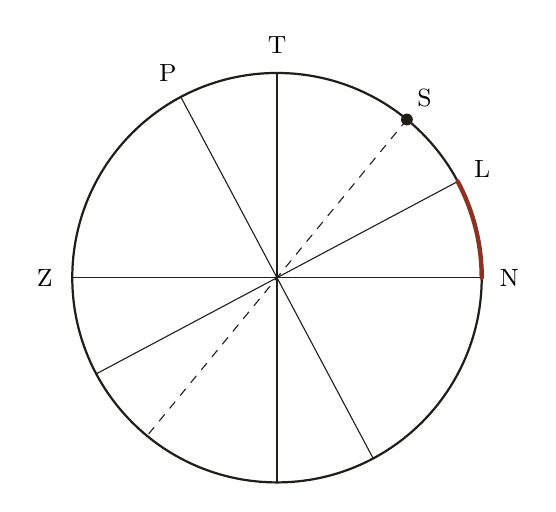
\begin{tikzpicture}[line cap=round,line join=round]
  \mscircle \msdiam{118.02} \msdiam{28.02}
  \msarc{0}{28.02}
  \mschord{50.6}{230.6} \msdot{50.6}
  \mslab{0}{N} \mslab{180}{Z} \mslab{90}{T}
  \mslab{118.02}{P} \mslab{28.02}{L} \mslab{50.6}{S}
\end{tikzpicture}
\mscaption{The circle turned about for a southern latitude: the elevated pole P now stands above Z and the equator L above N. S is the sun on the meridian, north of the zenith; the red arc NL, the equator's height, is what the working finds.}
\end{msfigure}

\dutchtext{Den 5 Januarij 1786, Jmand gissende met zijn Oog 15 Voet Booven den Zee te zijn,\footnote{\textit{Gissende met zijn oog 15 voet booven den zee te zijn} --- reckoning his eye to be fifteen feet above the sea. The datum is there to be subtracted: see the note.} schiet de Zon van vooren,\footnote{\textit{Van vooren} --- facing the sun, a fore-observation, as against the back-observation with the quadrant held over the shoulder.} en vind de zelve 50 gr: 40 men: Booven de Noord horisond te zijn; vrage na de Breete van de plaas. \textcolor{msred}{Antwoord, op 61 gr: 59 men: Zuijder Breete.}}
\engtext{On 5 January 1786, someone reckoning his eye to be 15 feet above the sea shoots the sun before him, and finds her to be 50 degrees 40 minutes above the north horizon; asked, the latitude of the place. \textit{Answer: 61 degrees 59 minutes south latitude.}}

\worktitle{Bewerking}{Working}
\begin{workblock}
  \wrow{}{\ang{22}{35} $=$ SL}{The sun's declination for the day, south.}
  \wrow{}{\ang{50}{36} $=$ SN}{Her height, the fifteen-foot eye taken off.}\ruleunder
  \wrow{}{\ang{28}{01} $=$ NL}{What is left is the equator's height above N.}
  \wrow{}{\ang{90}{00}}{}\ruleunder
  \wrow{}{\ang{61}{59} $=$ ZP}{\textit{off de Zuijder Breete} --- or the south latitude.}
\end{workblock}

\reading{South of the line the whole construction turns about: the pole that shows is the south one, standing above Z, and the equator crosses north of the zenith, above N. The sun on 5 January has south declination, so at this latitude she culminates to the north of the zenith and her height above N exceeds the equator's by exactly her declination. Take the one from the other and the equator's height above N is left; its complement is the height of the pole above Z, which is the latitude. One subtraction, one complement --- but the altitude that enters the working is not the altitude that was observed.}

\begin{msnotes}
  \item[2.] The question gives \ang{50}{40} and the working uses \ang{50}{36}. The four minutes are the dip of the horizon for an eye fifteen feet up, which is \ang{}{4.1} on the ordinary rule. The correction is made silently; only the fifteen feet in the question betray it.
  \item[5.] The sun's declination on 5 January 1786 was \ang{22}{34.4} south, against the table's \ang{22}{35}. The latitude, though, is another of the examiner's impossible places --- \ang{61}{59} south is deep in the Southern Ocean, far below any track the Company sailed.
\end{msnotes}

\mssection{Van het Verbeeteren der Zons Declinatie}{Of the correcting of the sun's declination}

% ---------------------------------------------------------------
\exempel{6de Exempel}{Sixth Example}

\dutchtext{Anno 1787, den 30 Augustus; Begeerd Men te Weeten de Zons Declinatie op 127 Graade en 30 Menuten, lengte, op de middag. \textcolor{msred}{Antwoord: 9 gr: 6 Men: Noorder Declinatie.}}
\engtext{In the year 1787, on the 30th of August, it is desired to know the sun's declination in 127 degrees 30 minutes of longitude, at noon. \textit{Answer: 9 degrees 6 minutes north declination.}}

\worktitle{Bewerking}{Working}
\begin{workblock}
  \wrow{Augustus d\textsuperscript{n} 29}{\ang{9}{21}}{The sun's north declination that day.}
  \wrow{,,\ 30}{\ang{8}{59}}{And the next.}\ruleunder
  \wrow{Verschil}{\ang{0}{22}}{Her change in twenty-four hours.}
  \wprop{As the whole circle is to the day's change, so is the longitude to the correction sought}{$360^{\circ} : 22' \;::\; 105^{\circ}\,59' : 7'$}
  \wprop{}{$21600 \;\big)\; 6359 \times 22 = 139898$}
  \wrow{}{\ang{0}{7}}{The correction.}
  \wrow{}{\ang{8}{59}}{The declination for the thirtieth.}\ruleunder
  \wrow{}{\ang{9}{6}}{\textit{Noorder Declinatie.}}
\end{workblock}

\reading{A declination table is computed for one meridian and for noon. A ship east of that meridian keeps its noon earlier, and by then the sun's declination has not yet fallen as far as the table says it will; so the day's change is divided in the ratio of the longitude to the whole circle, and the part is put back. The examiner reduces both terms to minutes, multiplies, divides by the minutes in a circle, and adds. What he does not write down is the step before all this: the longitude he divides with is not the longitude the question gave him.}

\begin{msnotes}
  \item[4.] The question says \ang{127}{30} and the working takes \ang{105}{59}, a silent reduction of \ang{21}{31}. That is the interval between the Peak of Tenerife, from which longitude at sea was reckoned, and Amsterdam, for whose meridian the table is computed: \ang{16}{38} west and \ang{4}{53} east make \ang{21}{31} exactly.
  \item[5.] The division comes to 6\vfrac{1}{2} minutes and he carries 7. The table itself is good: the sun's declination on those two days was \ang{9}{19.7} and \ang{8}{58.2}, a change of \ang{}{21.5} against his 22.
\end{msnotes}

\foliomark{3615 verso}{0050}{7--8}
\foliostand{The length of the day \textperiodcentered{} the error of the compass}{The seventh example is the only one on the paper worked in logarithms; with the eighth the section leaves the meridian for the horizon.}

% ---------------------------------------------------------------
\exempel{7de Exempel}{Seventh Example}

\begin{msfigure}
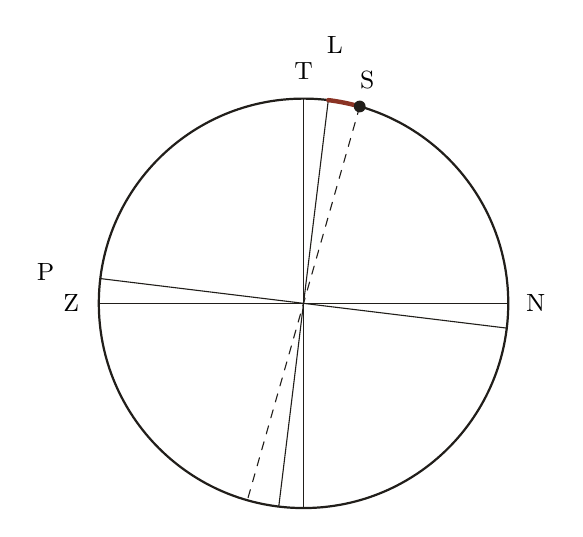
\begin{tikzpicture}[line cap=round,line join=round]
  \mscircle \msdiam{173.05} \msdiam{83.05}
  \msarc{74.07}{83.05}
  \mschord{74.07}{254.07} \msdot{74.07}
  \mslab{0}{N} \mslab{180}{Z} \mslab{90}{T}
  \mslab[3.3]{173.05}{P} \mslab[3.3]{83.05}{L} \mslab{74.07}{S}
\end{tikzpicture}
\mscaption{Samarang lies seven degrees south of the line, so the whole construction crowds into the zenith: P is barely clear of Z, and T, L and S stand within sixteen degrees of one another. The red arc LS is the sun's declination.}
\end{msfigure}

\dutchtext{Samarang is Leggende op 6 gr: 57 men Zuijder Breete; vrage hoe Lang het Dag, en Nagt zal Zijn, als de Zon 8 gr: 59 men: Noorder Declinatie heeft. \textcolor{msred}{Antwoord 11 uure 51 men: en 12 Seconde dag, en 12 uure 8 men: en 48 Seconde nagt.}}
\engtext{Samarang lies in 6 degrees 57 minutes south latitude; asked, how long the day and the night will be when the sun has 8 degrees 59 minutes north declination. \textit{Answer: 11 hours 51 minutes 12 seconds of day, and 12 hours 8 minutes 48 seconds of night.}}

\worktitle{Bewerking}{Working}
\begin{workblock}
  \wprop{Radius is to the tangent of the sun's declination as the tangent of the pole's height is to the sine of her rising and setting before or after six o'clock}{$1{,}000{,}000 \;:\; \tan 8^{\circ}59' \;::\; \tan 6^{\circ}57' \;:\; \sin x$}
  \wrow{}{$919889$}{The log tangent of the declination.}
  \wrow{}{$908600$}{The log tangent of the latitude.}\ruleunder
  \wrow{}{$1828489 =$ \ang{1}{06}}{Its log sine: how far from six o'clock the sun rises.}
  \wprop{As fifteen degrees are to one hour, so is that arc to the time}{$15^{\circ} \;:\; 1^{\mathrm{h}} \;::\; 1^{\circ}6' \;:\; 0^{\mathrm{h}}\,4^{\mathrm{m}}\,24^{\mathrm{s}}$}
  \wrow{}{\phantom{1}6 --- \phantom{1}0 --- \phantom{1}0}{}
  \wrow{}{\phantom{1}0 --- \phantom{1}4 --- 24}{}\ruleunder
  \wrow{}{\phantom{1}6 --- \phantom{1}4 --- 24}{\textit{de Sons opgang}}
  \wrow{}{12 --- \phantom{1}8 --- 48}{\textit{de Lengte van de Nagt}}
  \wrow{}{24 --- \phantom{1}0 --- \phantom{1}0}{}\ruleunder
  \wrow{}{11 --- 51 --- 12}{\textit{de Lengte van de Dag}}
\end{workblock}

\reading{On the equator the sun rises at six whatever her declination; away from it she rises before or after six by an arc that depends on both her declination and the latitude, and the rule for that arc --- the tangent of the one by the tangent of the other --- is the one piece of trigonometry the section uses. Here the latitude is south and the declination north, so the sun rises late and the day is the shorter of the two. Turn the arc into time at fifteen degrees to the hour, double it about six o'clock for the night, and take that from the whole day.}

\begin{msnotes}
  \item[1.] The rule is set down in the reckoning-school shorthand, \textit{R:s : T:s van de Z:s D:cl: $=$ T: P:s H:te : S:s van de Z:ons op en ondergang voor of na 6 uure} --- Radius, Tangens, Declinatie, Polus Hoogte, Sinus, each cut to its initial.
  \item[2.] The two figures are logarithms with the characteristic run into the mantissa, and they are exact: log tan \ang{8}{59} is 9\textperiodcentered19889 and log tan \ang{6}{57} is 9\textperiodcentered08600, to all five places he gives. The arc comes to \ang{1}{06.3} and the day to 11\textsuperscript{h}51\textsuperscript{m}12\textsuperscript{s}, which is his answer to the second.
  \item[3.] Samarang is put at \ang{6}{57} south. The town lies at \ang{6}{58}, so the school knew its own latitude to a minute --- the only place on the paper whose position can be checked against the map rather than the sky.
\end{msnotes}

% ---------------------------------------------------------------
\exempel{8ste Exempel}{Eighth Example}

\begin{msfigure}
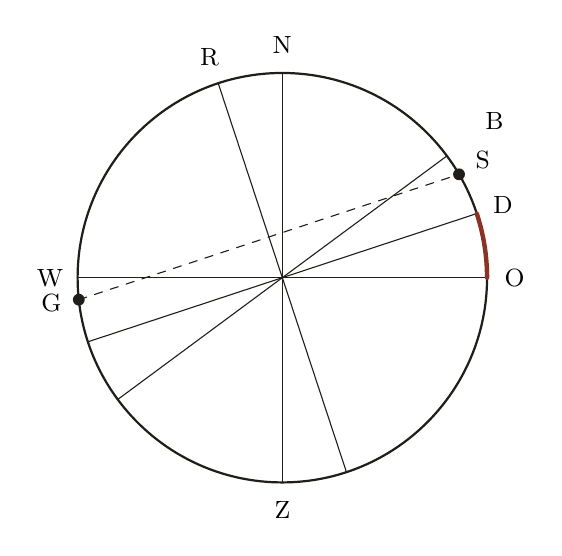
\begin{tikzpicture}[line cap=round,line join=round]
  \mscircle \msdiam{108.25} \msdiam{18.25} \msdiam{36.5}
  \msarc{0}{18.25}
  \mschord{186.17}{30.33} \msdot{30.33} \msdot{186.17}
  \mslab{90}{N} \mslab{270}{Z} \mslab{180}{W} \mslab{0}{O}
  \mslab{108.25}{R} \mslab{18.25}{D} \mslab{30.33}{S} \mslab[3.35]{36.5}{B} \mslab{186.17}{G}
\end{tikzpicture}
\mscaption{The horizon, seen from above. N, O, Z and W are the compass points and R and D the true north and east; S and G are the sun's observed rising and setting. The red arc DO is the variation, and it is also the arc NR.}
\end{msfigure}

\dutchtext{Jmand peijld de Zon in 't opkoome 30 Graade 20 Men: Benoorden het oost, en s'avons in 't ondergaan 6 graade 10 Men: Bezuijde het West; vraage na de misswijsing\footnote{\textit{Misswijsing} --- mis-pointing, the variation of the compass; \textit{Noord oostering} and \textit{Noord Westering} name its direction, easterly and westerly. \textit{Peijlen} is to take a bearing.} van het Compas. \textcolor{msred}{Antwoord 18 graade 15 menuten Noord oostering.}}
\engtext{Someone bears the sun at her rising 30 degrees 20 minutes north of east, and in the evening at her setting 6 degrees 10 minutes south of west; asked, the variation of the compass. \textit{Answer: 18 degrees 15 minutes north-easting.}}

\worktitle{Bewerking}{Working}
\begin{workblock}
  \wrow{}{\ang{30}{20} $=$ SO}{The rising, north of the compass east.}
  \wrow{Addeert}{\ang{6}{10} $=$ GW off BS}{The setting, south of the compass west.}\ruleunder
  \wrow{Komt}{\ang{36}{30} $=$ BO}{Laid off beyond S, it reaches B.}\ruleunder
  \wrow{2 $\big)$}{\ang{18}{15} $=$ DO off NR}{Half of it: the true east, and the variation.}
\end{workblock}

\reading{Wherever the sun rises north of east she sets as far north of west, the two amplitudes being equal about the true east--west line; and the compass, being wrong by a constant, adds its error to the one and takes it from the other. So the two observed departures do not agree, and half their sum is the amount by which the compass is out. The figure makes the argument visible: lay the setting's departure off beyond the rising's, bisect the whole, and the bisector D is where east really lies --- which is the same as saying that true north lies at R, \ang{18}{15} west of the compass north.}

\begin{msnotes}
  \item[4.] Halving gives the variation; the other half of the figure gives what was not asked for --- the sun's true amplitude, \ang{12}{05} north of east, from which her declination for the day could be recovered. The last two lines stand at the head of the next folio, above the ninth example, the leaf having run out beneath the question.
\end{msnotes}

\foliomark{3616}{0050}{9--10}
\foliostand{Courses and bearings corrected for the variation}{The paper ends where a steersman's day begins: with the compass in front of him and a correction to apply to it.}

% ---------------------------------------------------------------
\exempel{9de Exempel}{Ninth Example}

\begin{msfigure}
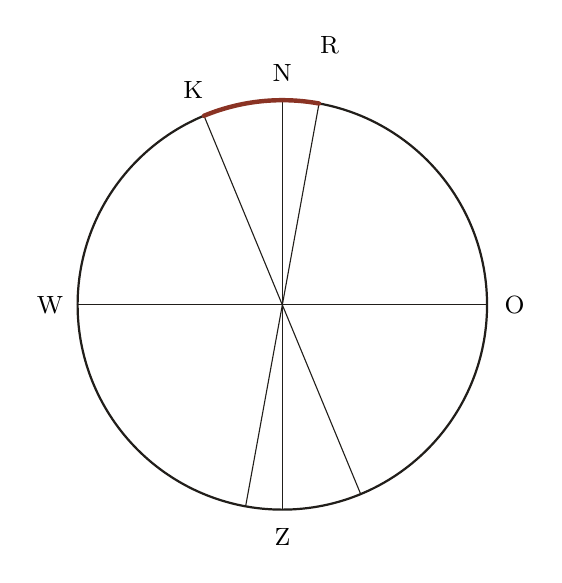
\begin{tikzpicture}[line cap=round,line join=round]
  \mscircle \msdiam{79.67} \msdiam{112.5}
  \msarc{79.67}{112.5}
  \mslab{90}{N} \mslab[3.35]{79.67}{R} \mslab{112.5}{K}
  \mslab{270}{Z} \mslab{0}{O} \mslab{180}{W}
\end{tikzpicture}
\mscaption{N is the compass north and R the true north, \ang{10}{20} east of it; K is the course steered. The red arc RK is what the question asks for --- the course as a true compass would show it.}
\end{msfigure}

\dutchtext{Indien men, Noord, Noord West, Zeijlde, op een Compas dat 10 gr: 20 men: Noorde Westering heeft; vrage wat Coers behoud men op Een Regtwijsend Compas.\footnote{\textit{Regtwijsend} --- right-pointing, a compass free of variation. \textit{Behouden coers} is the course actually kept, as against the course steered.} \textcolor{msred}{Antwoord N: W: ten Noorde 0 graade 55 men: Noordelijker.}}
\engtext{If one sailed north-north-west by a compass that has 10 degrees 20 minutes of north-westing, asked, what course is kept on a true compass. \textit{Answer: north-west by north, 0 degrees 55 minutes more northerly.}}

\worktitle{Bewerking}{Working}
\begin{workblock}
  \wrow{}{\ang{22}{30} $=$ NK}{North-north-west: two points from the compass north.}
  \wrow{Addeert}{\ang{10}{20} $=$ NR}{The variation, westerly.}\ruleunder
  \wrow{}{\ang{32}{50} $=$ RK}{The course reckoned from the true north.}
  \wrow{}{\ang{33}{45}}{\textit{Noord West ten Noorden} --- three points.}\ruleunder
  \wrow{}{\ang{0}{55}}{\textit{Noordelijker als Noord West ten Noorden.}}
\end{workblock}

\reading{A westerly variation carries the compass north round to the west, so a course steered by that card lies further west of the true north than the card says --- and the two quantities simply add. The interest is in the last two lines, which do not simplify the answer but complicate it: having got a clean \ang{32}{50} the examiner names the nearest point of the rose, north-west by north, and gives the remainder from it. That is not arithmetic but seamanship. Nobody steers \ang{32}{50}; a man at the wheel is given a point and told how much to favour one side of it.}

\begin{msnotes}
  \item[1.] The rose is of thirty-two points, so a point is \ang{11}{15} and every figure in this example and the next is a multiple or a part of it: two points to north-north-west, three to north-west by north.
\end{msnotes}

% ---------------------------------------------------------------
\exempel{10de Exempel}{Tenth Example}

\begin{msfigure}
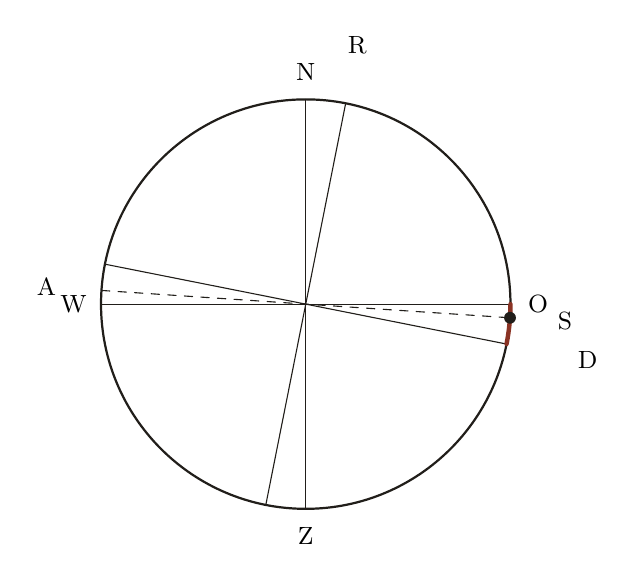
\begin{tikzpicture}[line cap=round,line join=round]
  \mscircle \msdiam{78.75} \msdiam{348.75}
  \msarc{348.75}{360}
  \mschord{176.17}{356.17} \msdot{356.17}
  \mslab{90}{N} \mslab[3.35]{78.75}{R} \mslab{270}{Z} \mslab{180}{W}
  \mslab[3.3]{176.17}{A} \mslab{0}{O} \mslab[3.3]{356.17}{S} \mslab[3.65]{348.75}{D}
\end{tikzpicture}
\mscaption{The same horizon. S is the sun's observed rising, D the true east; both fall south of the compass east O, and the red arc DO between them is the variation.}
\end{msfigure}

\dutchtext{De Zon in 't op koomen gepijld 3 graade 50 men: Bezuijden 't oost, en de Waare op komst\footnote{\textit{De waare opkomst} --- the true rising, that is the amplitude the sun's declination requires, taken from a table rather than from the compass.} is 7 graade 25 menuten Benoorden 't oost, vrage na de miswijsing. \textcolor{msred}{Antwoord 11 graade 15 menuten Noord Westering.}}
\engtext{The sun at her rising borne 3 degrees 50 minutes south of east, and the true rising being 7 degrees 25 minutes north of east; asked, the variation. \textit{Answer: 11 degrees 15 minutes north-westing.}}

\worktitle{Bewerking}{Working}
\begin{workblock}
  \wrow{}{\ang{3}{50} $=$ SO}{The bearing taken, south of the compass east.}
  \wrow{Addeert}{\ang{7}{25} $=$ DS}{The true rising, north of it.}\ruleunder
  \wrow{}{\ang{11}{15} $=$ DO off NR}{The whole distance between them: the variation.}
\end{workblock}

\reading{The eighth example found the variation from two observations and no table; this one finds it from one observation and a table, and is three lines long. The sun's true amplitude being known, the compass's error is simply the angle between where she rose and where she should have risen --- and since the one falls south of east and the other north of it, the two are added. It is the shortest working in the section and the last, and the paper closes on a figure a steersman could have read off his card without any working at all.}

\begin{msnotes}
  \item[3.] \ang{11}{15} is one point of the compass exactly. Every other answer in the section is an awkward number; the examiner ends on one that a man could set on his card by eye, and says nothing about it.
\end{msnotes}

\end{document}
